\documentclass[10pt,twocolumn,letterpaper]{article}

% CVPR-style formatting and fonts
\usepackage{cvpr}
\usepackage{mathptmx} % Remplace l'ancien package 'times'
\usepackage{microtype} % Règle automatiquement les espacements disgracieux
\usepackage{epsfig}
\usepackage{graphicx}
\usepackage{amsmath}
\usepackage{amssymb}
\usepackage{url}
\usepackage{siunitx}
\sisetup{group-separator = {\,}, group-minimum-digits=4}
\usepackage{booktabs}
\usepackage{subcaption}
\usepackage{caption}
\captionsetup{compatibility=false}
\usepackage{tabularx}
\usepackage{authblk}
\usepackage{tikz}
\usetikzlibrary{arrows.meta,positioning}
\usepackage{placeins}
\setlength{\emergencystretch}{2em}
% WCAG-friendly light fills (dark text contrast)
\definecolor{BackendTorch}{RGB}{224,236,247}
\definecolor{BackendCuda}{RGB}{226,242,233}
\definecolor{BackendNumpy}{RGB}{242,244,247}
\definecolor{BackendSVM}{RGB}{233,245,233}

\newcolumntype{Y}{>{\raggedright\arraybackslash}X}

\cvprfinalcopy
\def\cvprPaperID{****}
\def\httilde{\mbox{\tt\raisebox{-.5ex}{\symbol{126}}}}
\ifcvprfinal\pagestyle{empty}\fi

\begin{document}

\title{Project Work Parallel Programming: \\ Acceleration of Quantum Kernel Methods for Image Classification Tasks}

\author{Fouepe Dylan\\
{\tt\small dylan.fouepe@edu.unifi.it}}
\affil{University of Florence}

\maketitle
\thispagestyle{empty}

\begin{abstract}
This project studies binary SVM training on classical image datasets using simulated quantum kernels, 
with a strong focus on parallel programming and heterogeneous CPU/GPU optimization. 
The project repository provides three execution paths: a classical CPU baseline, a GPU quantum backend 
based on PennyLane+PyTorch (\textbf{GPU base}), and a custom HPC backend (\textbf{GPU custom}) built on CuPy, 
DLPack, and a bespoke C++ CUDA kernel. The core of the work is to build quantum Gram matrices of size $N \times N$ 
quickly and correctly, whose cost remains $O(N^2 \cdot 2^Q)$ for $Q$ qubits.

Experiments on Fashion-MNIST, CIFAR-10, and SVHN reveal two regimes. On Fashion-MNIST, the quantum kernel 
remains strong in the latest run-scoped campaign, with values up to \textbf{F1 = 0.9653} and 
\textbf{AUC = 0.9956} (\textbf{GPU base}, size 1000). On CIFAR-10 and SVHN, however, kernels tend to concentrate, 
the inter-class gap becomes nearly zero, and the SVM often ends with a support-vector fraction close to $1.0$, 
consistent with a \emph{kernel collapse} or \emph{barren-plateau-like} behavior. Overall, the reported 
results provide a consistent comparison of throughput and predictive quality across classical and 
quantum-kernel settings.
\end{abstract}

\section{Introduction}
Quantum kernel methods provide a clean way to project classical data into a very high-dimensional Hilbert space 
and then solve a classification task with a precomputed SVM~\cite{havlicek2019supervised}. 
In practice, this promise quickly runs into a cost bottleneck: for $N$ samples and $Q$ qubits, building 
the Gram matrix requires simulating states of dimension $2^Q$ and evaluating $O(N^2)$ complex overlaps. 
At $Q=16$ a single state vector already contains $65{,}536$ complex amplitudes.

The study compares a classical SVM baseline and two quantum-kernel backends under the same experimental protocol. 
The report focuses on comparative evidence: predictive quality (F1/AUC), runtime, throughput, 
and failure indicators related to kernel concentration.

\section{Scope of the Project}
This study addresses three questions:
\begin{itemize}
    \item How do classical and quantum-kernel SVMs compare on the same binary tasks?
    \item Which backend provides the best throughput/runtime trade-off at 16 qubits?
    \item Which empirical signals indicate kernel concentration and reduced separability?
\end{itemize}

The analysis focuses on measurable outcomes: F1, AUC, runtime, throughput, and kernel-shape diagnostics.

\section{Experimental Methodology}
Three datasets are used for binary classification: Fashion-MNIST~\cite{xiao2017fashion}, 
CIFAR-10~\cite{krizhevsky2009cifar}, and SVHN~\cite{netzer2011svhn}. 
Each is binarized into three tasks of increasing difficulty (see Table~\ref{tab:tasks}).

\textbf{Hardware Setup:} All benchmarks and training pipelines were executed on a dedicated HPC node equipped 
with an AMD EPYC 7343 16-Core Processor and a NVIDIA RTX 6000 Ada Generation GPU (48\,GB VRAM). The environment 
relies on CUDA 13.1, providing massive parallelism for both the native PyTorch and custom CUDA backends.
All experiments use $Q=16$ qubits by default, yielding state vectors of dimension $2^{16} = 65{,}536$ 
complex amplitudes. Key performance observations from the benchmark campaign at this scale are:
\begin{itemize}
    \item at 16 qubits, the direct backend comparison places \textbf{GPU custom} ahead of both \textbf{CPU base} 
    and \textbf{GPU base} in throughput;
    \item across the measured 16-qubit configurations, peak GPU memory remains in a moderate range
     (about \SI{0.06}{GB} to \SI{3.00}{GB}), indicating that throughput gains are not tied to extreme VRAM pressure.
\end{itemize}

\begin{table}[t]
\centering
\caption{Binary classification tasks configured in the repository.}
\label{tab:tasks}
\small
\begin{tabular}{llll}
\toprule
\textbf{Dataset} & \textbf{Easy} & \textbf{Med} & \textbf{Hard} \\
\midrule
Fashion-MNIST & 0 vs 1 & 3 vs 8 & 0 vs 6 \\
CIFAR-10 & 1 vs 6 & 0 vs 2 & 3 vs 5 \\
SVHN & 1 vs 0 & 2 vs 7 & 3 vs 5 \\
\bottomrule
\end{tabular}
\end{table}

From the quantum perspective, most configurations use $16$ PCA components (thus $16$ qubits) with a shallow 
circuit depth by default. Circuit layers are configurable via YAML through \textit{layer config}; 
an important case is a hard CIFAR-10 configuration, which forces \textbf{6 layers} and serves as 
a "hard" regime to observe kernel concentration.

\subsection{Preprocessing and Quantum Feature Map}
The training pipeline follows these steps:
\begin{enumerate}
    \item extract pixel values and flatten;
    \item apply PCA to $d=16$ components;
    \item scale features via \textit{range scaling};
    \item encode features using the \textit{angle map}, \textit{Y map} or \textit{YZ map};
    \item simulate states via PennyLane/\textit{state simulator}.
\end{enumerate}

The experiments use the \textbf{YZ ansatz} with entangling layers, which provides a simple trade-off 
between expressivity and simulation cost. Circuit weights are initialized once per run from a normal 
distribution and kept fixed during SVM training; this is therefore not a full variational 
training loop but a \emph{kernel-based} learning approach.

The target kernel is the fidelity kernel
\[
k(x_i, x_j) = \left|\langle \psi(x_i) \mid \psi(x_j) \rangle \right|^2.
\]
In practice, if $S_A \in \mathbb{C}^{N_A \times 2^Q}$ and $S_B \in \mathbb{C}^{N_B \times 2^Q}$ are 
the state matrices, then
\[
K_{ij} = \left| \sum_{k=1}^{2^Q} S_A[i,k]\;\overline{S_B[j,k]} \right|^2.
\]

\subsection{Training Protocol}
The experimental protocol uses:
\begin{itemize}
    \item train/test split inherited from the dataset;
    \item 3-fold cross-validation on the training partition;
    \item hyperparameter optimization of $C$ via Optuna~\cite{akiba2019optuna} 
    (sampling $C$ over a log-uniform distribution);
    \item final re-fit on train+val;
    \item final evaluation on the test set.
\end{itemize}

In addition to F1 and AUC, the analysis tracks runtime, support-vector fraction, and kernel distribution statistics 
to distinguish optimization effects from representational limits.

\section{HPC Architecture}
\subsection{Unified Backend API}

For Gram computation, we use a unified API that accepts the same data and normalization flags, 
but delegates execution to three paths:
\begin{itemize}
    \item \textbf{CPU base}: CPU fallback, useful as a reference and for small cases;
    \item \textbf{GPU base}: generate states and perform matrix computation directly on the GPU with PyTorch;
    \item \textbf{GPU custom}: generate states with PyTorch, convert tensors to CuPy via DLPack (enabling 
    efficient zero-copy memory sharing without CPU round-trips), and compute the Gram with a custom \textit{CUDA kernel}.
\end{itemize}
Figure~\ref{fig:backend-api} summarises the delegation flow from preprocessed features to the SVM solver.

\begin{figure}[t]
\centering
\resizebox{0.88\columnwidth}{!}{%
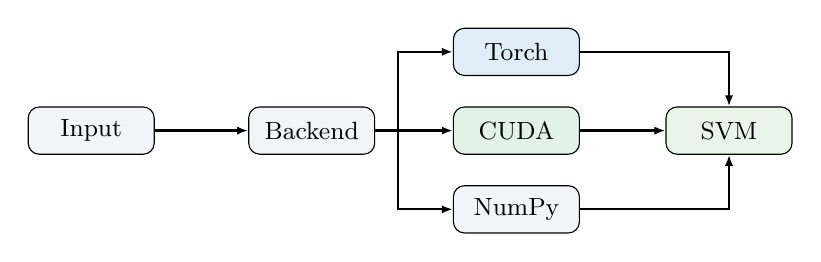
\begin{tikzpicture}[
        box/.style={draw, rounded corners, minimum width=1.6cm, minimum height=0.6cm,
                                align=center, font=\small},
        arr/.style={-{Latex[length=4pt]}, thick}
]
    \node[box, fill=BackendNumpy]  (data)  at (0,0)    {Input};
    \node[box, fill=BackendNumpy]  (router) at (2.8,0) {Backend};
    \node[box, fill=BackendTorch]  (torch) at (5.4,1.0)  {Torch};
    \node[box, fill=BackendCuda]   (cuda)  at (5.4,0)    {CUDA};
    \node[box, fill=BackendNumpy]  (numpy) at (5.4,-1.0) {NumPy};
    \node[box, fill=BackendSVM]    (svm)   at (8.1,0)   {SVM};
    \draw[arr] (data) -- (router);
    \draw[arr] (router) -- ++(1.1,0) |- (torch);
    \draw[arr] (router) -- (cuda);
    \draw[arr] (router) -- ++(1.1,0) |- (numpy);
    \draw[arr] (torch) -| (svm);
    \draw[arr] (cuda)  -- (svm);
    \draw[arr] (numpy) -| (svm);
\end{tikzpicture}%
}
\caption{Unified backend API: the Gram matrix is computed on GPU (\textbf{GPU base} or \textbf{GPU custom}) or CPU (\textbf{CPU base}); 
the SVM solver always runs on CPU.}
\label{fig:backend-api}
\end{figure}

\subsection{NumPy CPU Backend}
The \textbf{CPU base} backend runs Gram-matrix computation on CPU and serves as the baseline path for backend comparison.
It is used as a numerical reference and remains practical for smaller kernels where CPU overhead is limited.
Unlike the GPU backends, it does not rely on VRAM-aware tiling, stream orchestration, or autotuning.
Figure~\ref{fig:numpy-flow} illustrates its computation flow.

\subsection{Torch GPU Backend}
The \textbf{GPU base} backend uses native PyTorch GPU operations to generate states and compute Gram matrices. 
In this study, it is treated as the main GPU reference point for quality/runtime comparison against 
both \textbf{CPU base} and \textbf{GPU custom}.
Its distinctive optimizations are pinned host memory and CUDA streams, which target transfer overlap 
rather than custom kernel tuning.
Figure~\ref{fig:torch-flow} shows its internal flow.

\subsection{Custom CUDA Backend \textbf{GPU custom}}
The \textbf{GPU custom} backend computes Gram matrices with custom CUDA kernels through CuPy. 
In this report, its role is assessed through measured throughput and downstream classification metrics, 
not by internal kernel structure.
Figure~\ref{fig:cuda-flow} details its computation pipeline.

\begin{figure}[t]
\centering

\begin{subfigure}[t]{\columnwidth}
\centering
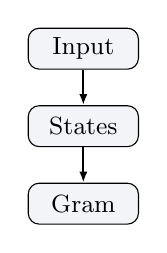
\begin{tikzpicture}[
    box/.style={draw, rounded corners, minimum width=1.4cm, minimum height=0.52cm,
                                align=center, font=\small},
    arr/.style={-{Latex[length=4pt]}, thick},
    node distance=0.45cm
]
    \node[box, fill=BackendNumpy] (feat) {Input};
    \node[box, fill=BackendNumpy, below=of feat] (states) {States};
    \node[box, fill=BackendNumpy, below=of states] (gram) {Gram};
    \draw[arr] (feat) -- (states);
    \draw[arr] (states) -- (gram);
\end{tikzpicture}
\caption{CPU base flow.}
\label{fig:numpy-flow}
\end{subfigure}

\vspace{0.4cm}

\begin{subfigure}[t]{\columnwidth}
\centering
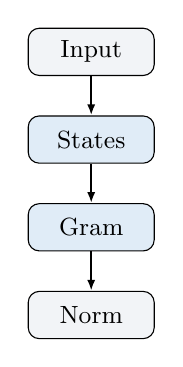
\begin{tikzpicture}[
    box/.style={draw, rounded corners, minimum width=1.6cm, minimum height=0.6cm,
                                align=center, font=\small},
    arr/.style={-{Latex[length=4pt]}, thick},
    node distance=0.5cm
]
    \node[box, fill=BackendNumpy]  (feat) {Input};
    \node[box, fill=BackendTorch, below=of feat]  (states) {States};
    \node[box, fill=BackendTorch, below=of states]  (gram) {Gram};
    \node[box, fill=BackendNumpy, below=of gram]  (norm) {Norm};
    \draw[arr] (feat) -- (states);
    \draw[arr] (states) -- (gram);
    \draw[arr] (gram) -- (norm);
\end{tikzpicture}
\caption{GPU base flow.}
\label{fig:torch-flow}
\end{subfigure}

\vspace{0.4cm}

\begin{subfigure}[t]{\columnwidth}
\centering
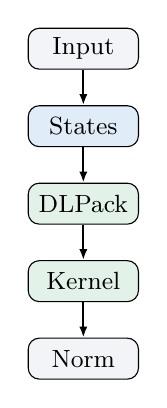
\begin{tikzpicture}[
    box/.style={draw, rounded corners, minimum width=1.4cm, minimum height=0.52cm,
                                align=center, font=\small},
    arr/.style={-{Latex[length=4pt]}, thick},
    node distance=0.45cm
]
    \node[box, fill=BackendNumpy]  (feat) {Input};
    \node[box, fill=BackendTorch, below=of feat]  (states) {States};
    \node[box, fill=BackendCuda, below=of states]   (dlpack) {DLPack};
    \node[box, fill=BackendCuda, below=of dlpack]   (rawker) {Kernel};
    \node[box, fill=BackendNumpy, below=of rawker]  (norm) {Norm};
    \draw[arr] (feat) -- (states);
    \draw[arr] (states) -- (dlpack);
    \draw[arr] (dlpack) -- (rawker);
    \draw[arr] (rawker) -- (norm);
\end{tikzpicture}
\caption{GPU custom flow.}
\label{fig:cuda-flow}
\end{subfigure}

\caption{Comparison of backend pipelines}
\label{fig:backend_comparison}
\end{figure}

\begin{figure}[t]
\centering

\begin{subfigure}[t]{0.28\columnwidth}
\centering
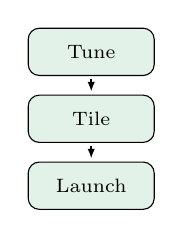
\begin{tikzpicture}[
        stage/.style={draw, fill=BackendCuda, rounded corners,
                    minimum width=1.6cm, minimum height=0.6cm, align=center, font=\scriptsize},
        arr/.style={-{Latex[length=3.6pt]}, line width=0.9pt, shorten >=1pt, shorten <=1pt}
]
    \node[stage] (s1) at (0,0) {Tune};
    \node[stage] (s2) at (0,-0.85) {Tile};
    \node[stage] (s3) at (0,-1.70) {Launch};
    \draw[arr] (s1) -- (s2);
    \draw[arr] (s2) -- (s3);
\end{tikzpicture}
\caption{Host flow.}
\end{subfigure}%
\hfill
\begin{subfigure}[t]{0.42\columnwidth}
\centering
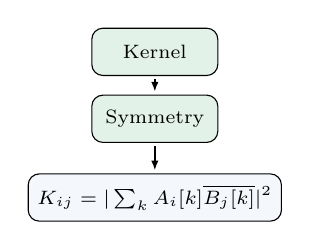
\begin{tikzpicture}[
        stage/.style={draw, fill=BackendCuda, rounded corners,
                    minimum width=1.6cm, minimum height=0.6cm, align=center, font=\scriptsize},
    note/.style={draw, rounded corners, fill=BackendTorch!35, minimum width=1.6cm, minimum height=0.6cm, align=center, font=\scriptsize},
        arr/.style={-{Latex[length=3.6pt]}, line width=0.9pt, shorten >=1pt, shorten <=1pt}
]
    \node[stage] (s4) at (0,0) {Kernel};
    \node[stage] (s5) at (0,-0.85) {Symmetry};
    \node[note] (eq) at (0,-1.85) {$K_{ij}=|\sum_k A_i[k]\overline{B_j[k]}|^2$};
    \draw[arr] (s4.south) -- (s5.north);
    \draw[arr] (s5.south) -- (eq.north);
\end{tikzpicture}
\caption{Device core.}
\end{subfigure}%
\hfill
\begin{subfigure}[t]{0.28\columnwidth}
\centering
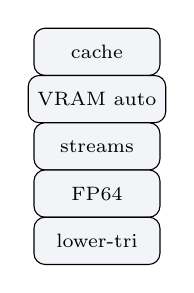
\begin{tikzpicture}[
    opt/.style={draw, rounded corners, fill=BackendNumpy, minimum width=1.6cm, minimum height=0.6cm, align=center, font=\scriptsize}
]
    \node[opt] (o1) at (0,0) {cache};
    \node[opt] (o2) at (0,-0.6) {VRAM auto};
    \node[opt] (o3) at (0,-1.2) {streams};
    \node[opt] (o4) at (0,-1.8) {FP64};
    \node[opt] (o5) at (0,-2.4) {lower-tri};
\end{tikzpicture}
\caption{Optimization.}
\end{subfigure}

\caption{Kernel construction in \textbf{GPU custom}, organized across three elements: host orchestration, device kernel core, and optimization controls.}
\label{fig:rawkernel}
\end{figure}

\subsubsection{Backend Optimizations}
Backend-specific optimizations are:
\begin{itemize}
    \item \textbf{GPU base path}: pinned host memory and CUDA streams are used to overlap transfer/compute stages, without custom CUDA kernel tuning.
    \item \textbf{VRAM-aware sizing}: state\_tile=-1 automatically sizes state block dimensions 
    according to available VRAM.
    \item \textbf{Autotuning}: CUDA kernel tile sizes are learned and cached persistently across runs.
     A specific entry for 16 qubits in double precision is handled.
    \item \textbf{Bulk precompute}: when memory permits, all states in a block are prebuilt to reduce round-trips and leverage GPU parallelism.
    \item \textbf{Stream pool}: multiple CUDA streams can be used to orchestrate state preparation and Gram computation.
    \item \textbf{Memory profiling}: the benchmark measures VRAM usage, transfers and throughput.
    \item \textbf{CPU base path}: Use smal state\_tile sizes to take advantage of CPU cache and avoid VRAM-like bottlenecks.
     The CPU path does not use pinned memory or streams, as these are GPU-specific optimizations.
     Instead, it relies on efficient NumPy operations and multi-threading where possible.
\end{itemize}

Benchmark ablations identify the most useful settings:
\begin{itemize}
    \item disabling precompute is the slowest option in the reported \textbf{GPU custom} ablation rows;
    \item vram\_fraction=0.95 is the selected optimum in each of the stored profile logs;
    \item num\_streams=1 is the selected optimum in the stored stream-sweep rows;
    \item torch\_pinned+streams is the best torch configuration in the stored torch ablation rows.
\end{itemize}

At this scale, data movement and memory organization have a larger effect than increasing stream complexity.

\subsubsection{Normalization and Metric Comparability}
All backends share the same post-processing and kernel normalization protocol so that F1/AUC and runtime differences can be interpreted as backend effects 
rather than normalization artifacts:
\begin{itemize}
    \item finite-value checks (NaN/Inf) before writing kernel blocks;
    \item diagonal validation before normalization and classifier fitting;
    \item shared kernel normalization across backends;
    \item strict cross-normalization
    \[
    \hat K(X,Y)_{ij} = \frac{K(X,Y)_{ij}}{\sqrt{K(X,X)_{ii}K(Y,Y)_{jj}}}
    \]
    applied after computing both diagonals;
    \item identical post-normalization path before SVM fitting and evaluation.
\end{itemize}

This shared normalization pipeline is the basis for fair backend-to-backend metric comparisons.

\section{Performance Results}
\subsection{Benchmark}
The benchmark captures qubit scaling, sample scaling, optimization ablations, tile-state tuning, VRAM-fraction sensitivity, 
stream-count impact, and kernel fidelity against the \textbf{CPU base} reference. 
The validations are run across the datasets with two warmup runs and two timed runs per point. Outputs include 
per-dataset benchmark summaries, figures, and execution logs.

\begin{table}[t]
\centering
\caption{Sample-scaling throughput (Mpairs/s) by dataset and backend from per-dataset benchmark CSVs. Values 
are reported at the highest sample-scaling qubit setting available in each dataset profile 
(Fashion: 12 qubits; CIFAR-10 and SVHN: 16 qubits).}
\label{tab:benchmark}
\scriptsize
\setlength{\tabcolsep}{4pt} % Légèrement augmenté car on a enlevé le resizebox
\begin{tabular}{llcccc}
\toprule
\textbf{Dataset} & \textbf{Size} & \textbf{Qubits} & \textbf{CPU base} & \textbf{GPU base} & \textbf{GPU custom} \\
\midrule
fashion & 256  & 12 & 0.0059 & 0.0140 & 0.0159 \\
fashion & 512  & 12 & 0.0224 & 0.0299 & 0.0298 \\
fashion & 1024 & 12 & 0.0856 & 0.0575 & 0.0546 \\
cifar10 & 256  & 16 & 0.0020 & 0.0057 & 0.0062 \\
cifar10 & 512  & 16 & 0.0086 & 0.0175 & 0.0112 \\
cifar10 & 1024 & 16 & 0.0319 & 0.0375 & 0.0245 \\
svhn    & 256  & 16 & 0.0023 & 0.0053 & 0.0058 \\
svhn    & 512  & 16 & 0.0097 & 0.0175 & 0.0124 \\
svhn    & 1024 & 16 & 0.0328 & 0.0366 & 0.0243 \\
\end{tabular}
\end{table}

Key observations from these benchmark statistics are:
\begin{itemize}
    \item at small sample sizes (256), GPU backends are consistently faster than NumPy across datasets;
    \item at 512 samples, \textbf{GPU base} is the fastest backend in all three dataset profiles;
    \item at 1024 samples, \textbf{GPU base} remains fastest on CIFAR-10 and SVHN, while \textbf{CPU base} is fastest on Fashion.
\end{itemize}

The benchmark plots in Figs.~\ref{fig:bench-fashion}, \ref{fig:bench-cifar10}, and \ref{fig:bench-svhn} are consistent with Table~\ref{tab:benchmark}: 
backend ranking depends on both dataset profile and sample size.

\begin{figure}[htbp]
\centering
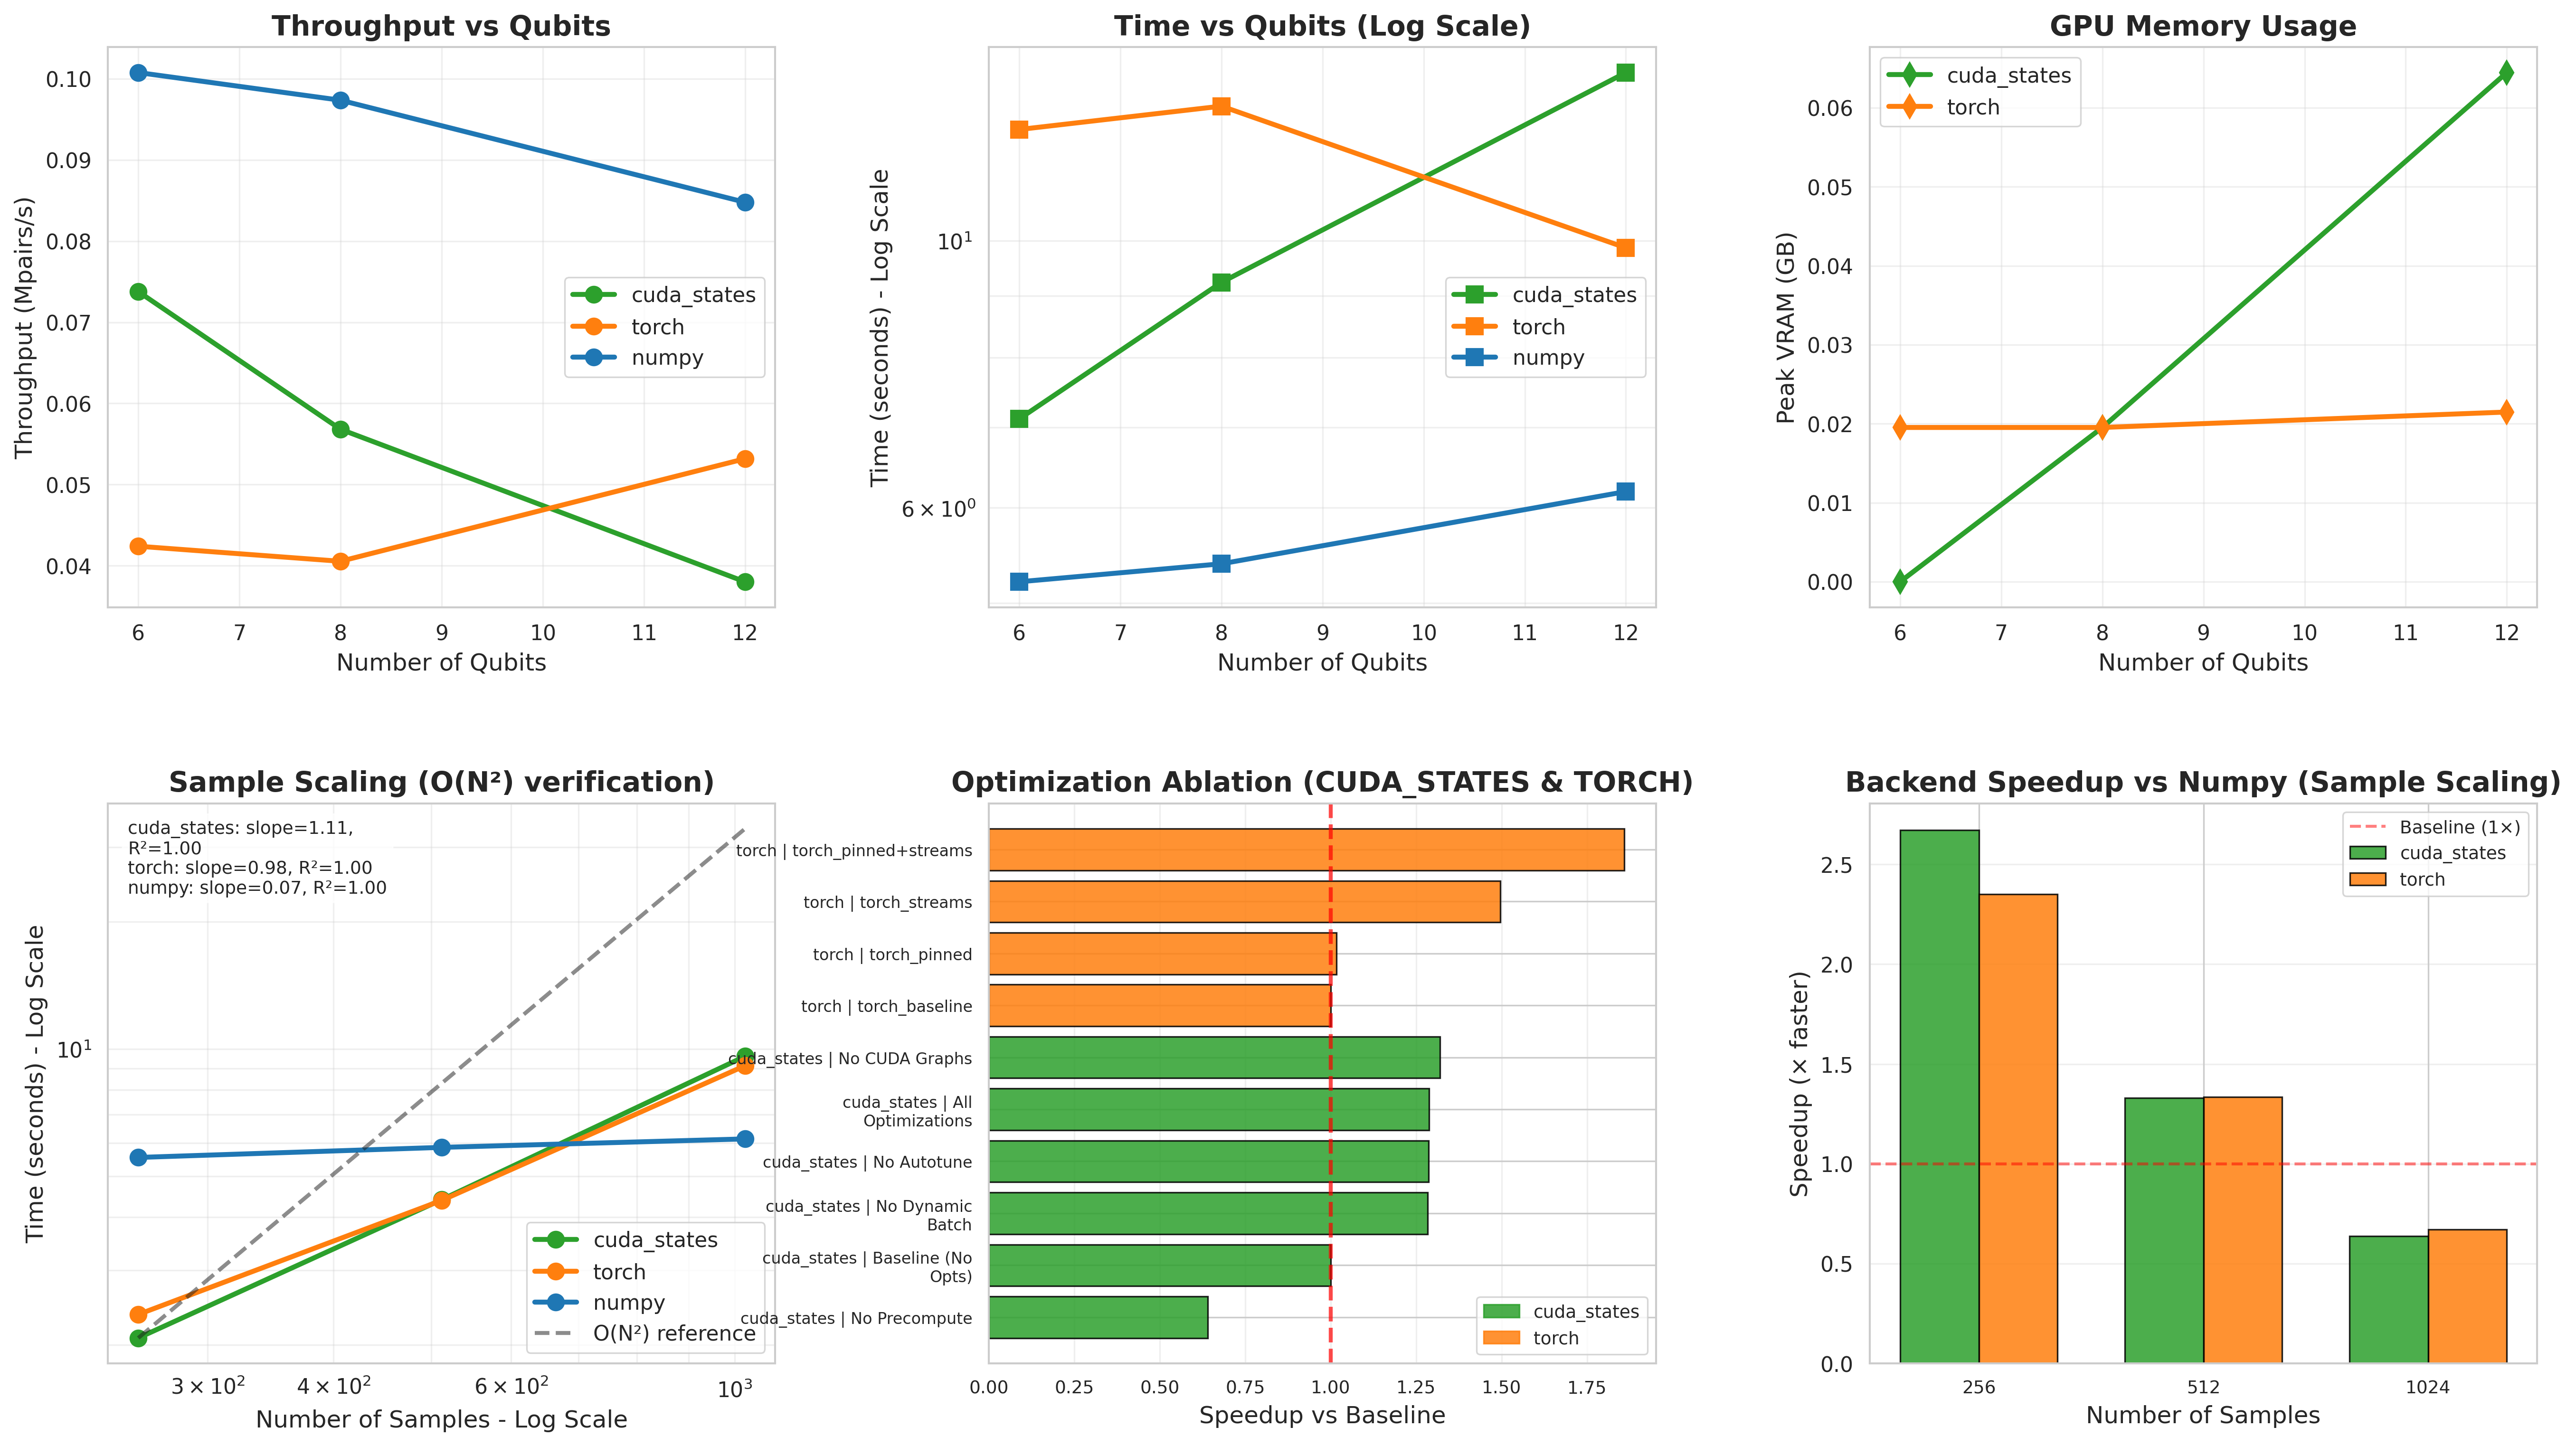
\includegraphics[width=\columnwidth]{benchmark_results/fashion/benchmark.png}
\caption{Fashion-MNIST benchmark profile.}
\label{fig:bench-fashion}
\end{figure}

\begin{figure}[htbp]
\centering
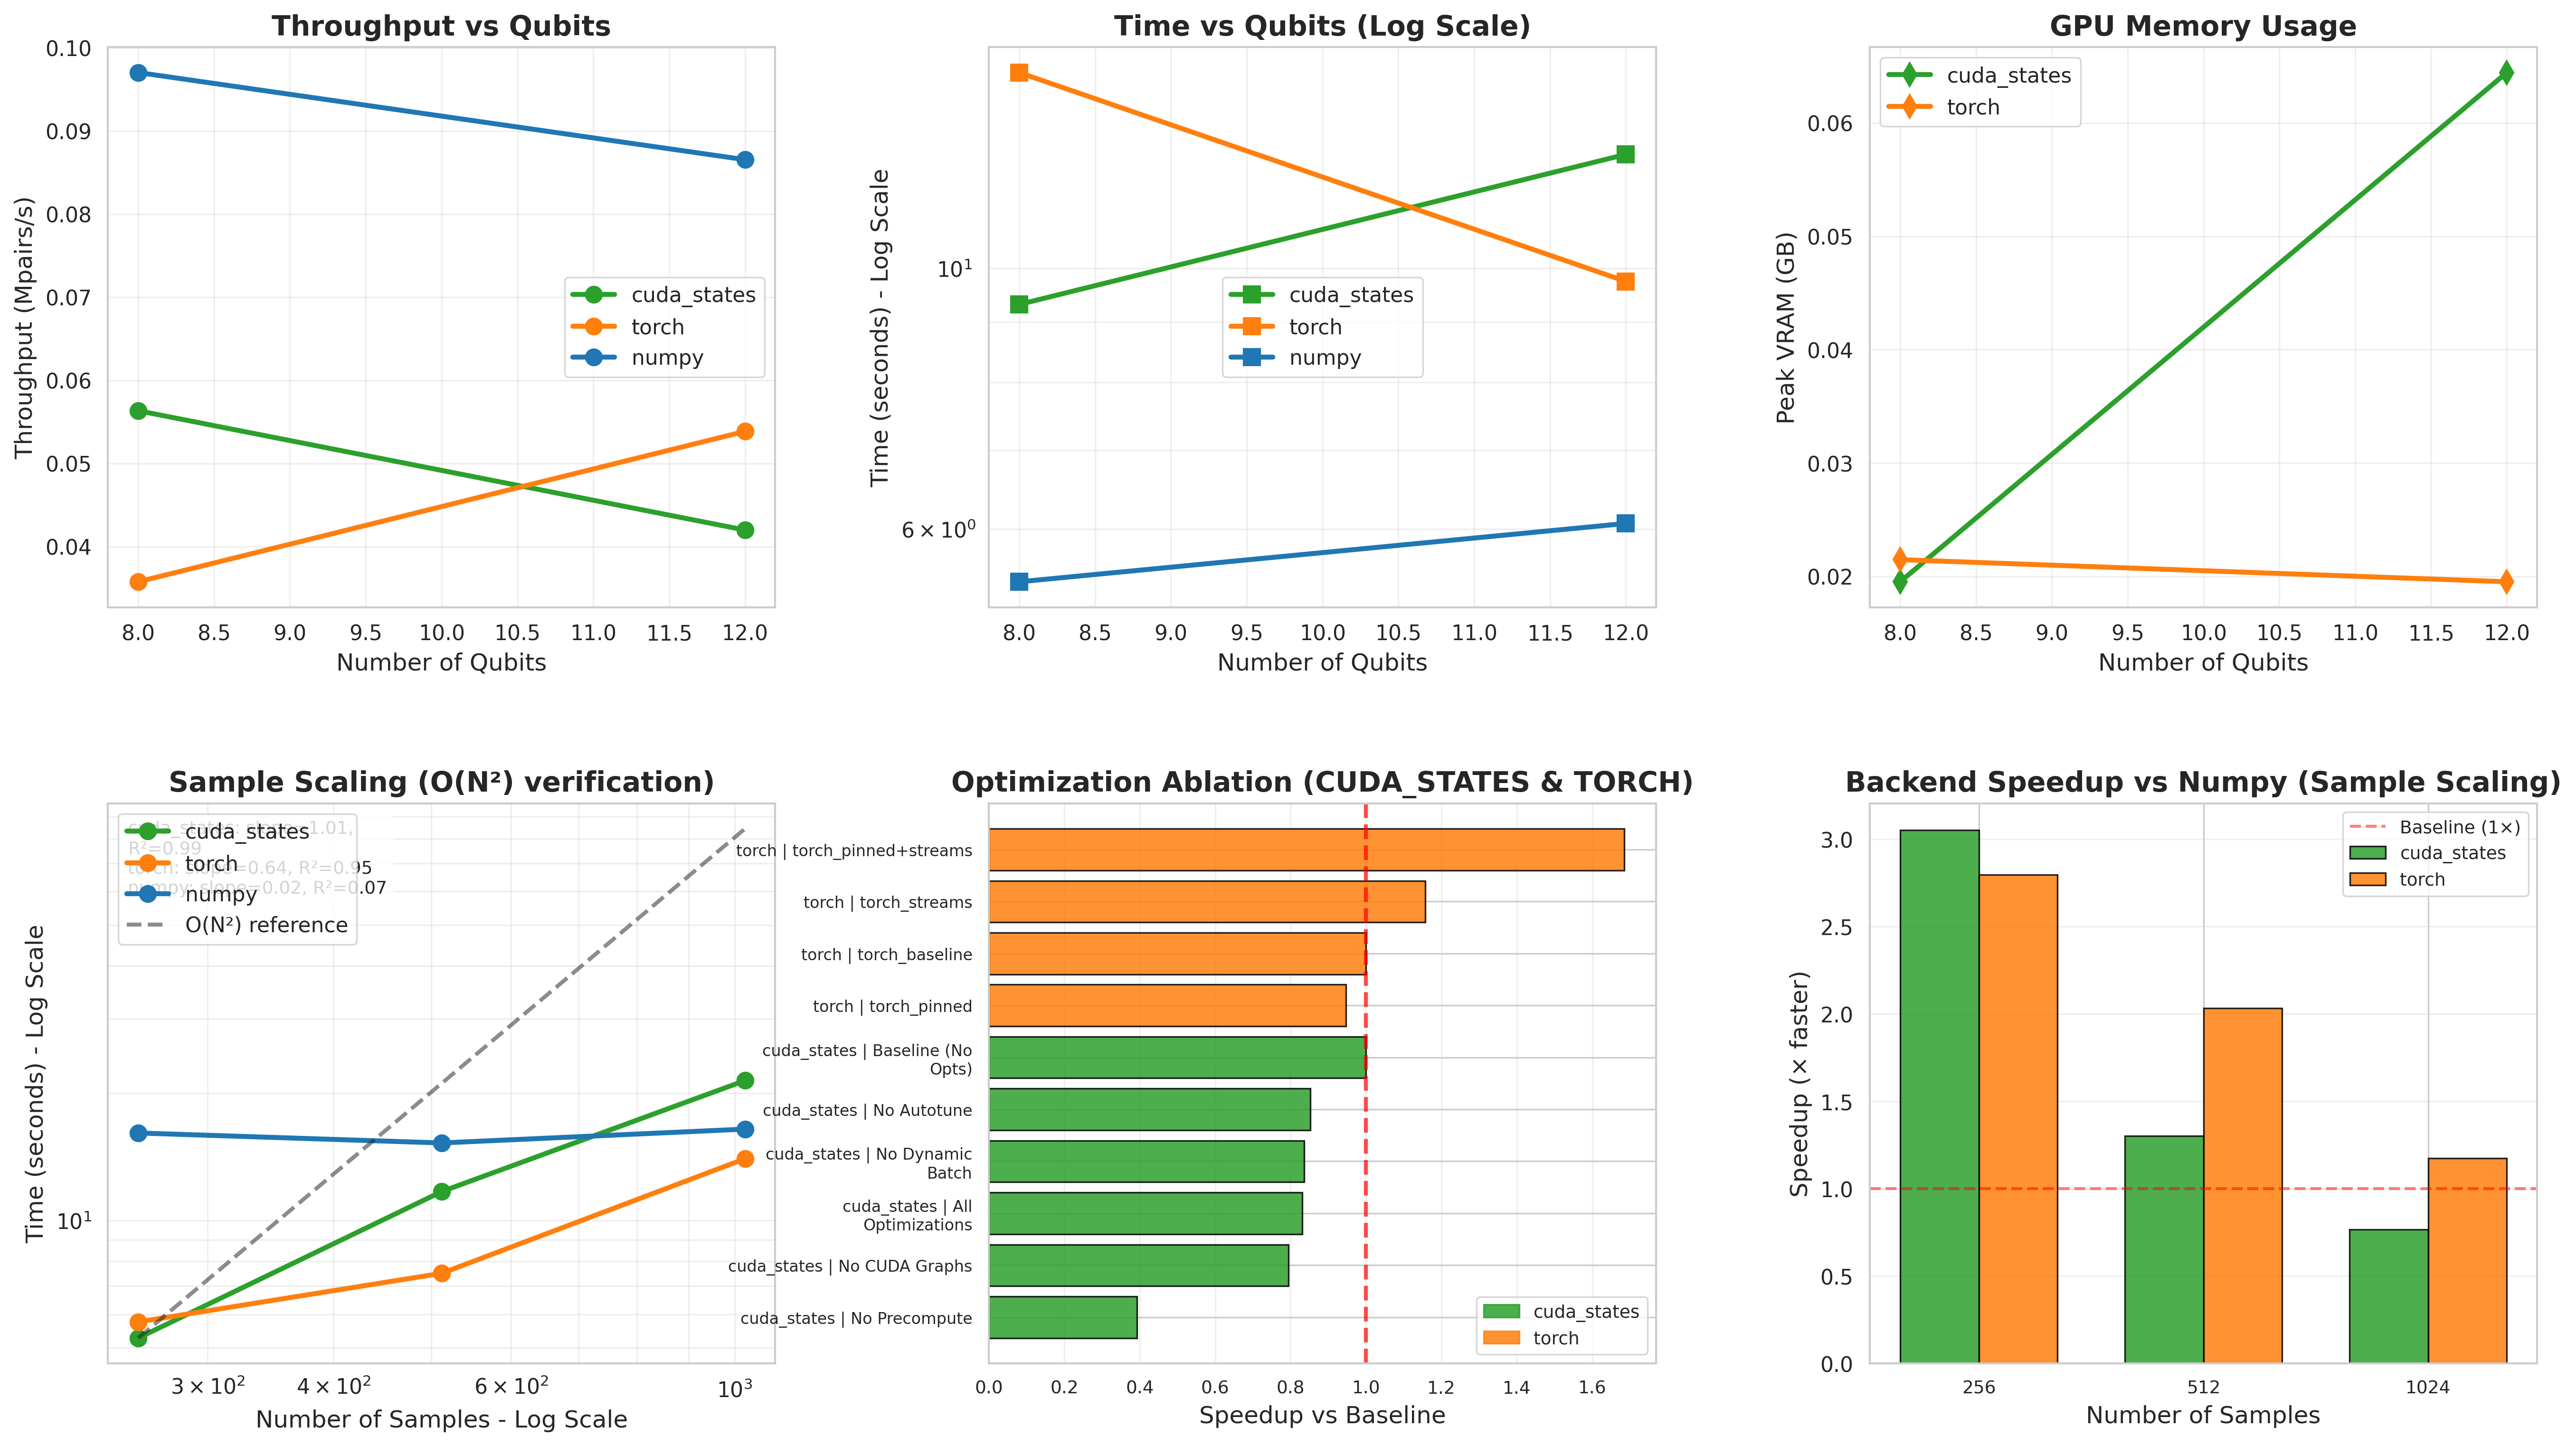
\includegraphics[width=\columnwidth]{benchmark_results/cifar10/benchmark.png}
\caption{CIFAR-10 benchmark profile.}
\label{fig:bench-cifar10}
\end{figure}

\begin{figure}[htbp]
\centering
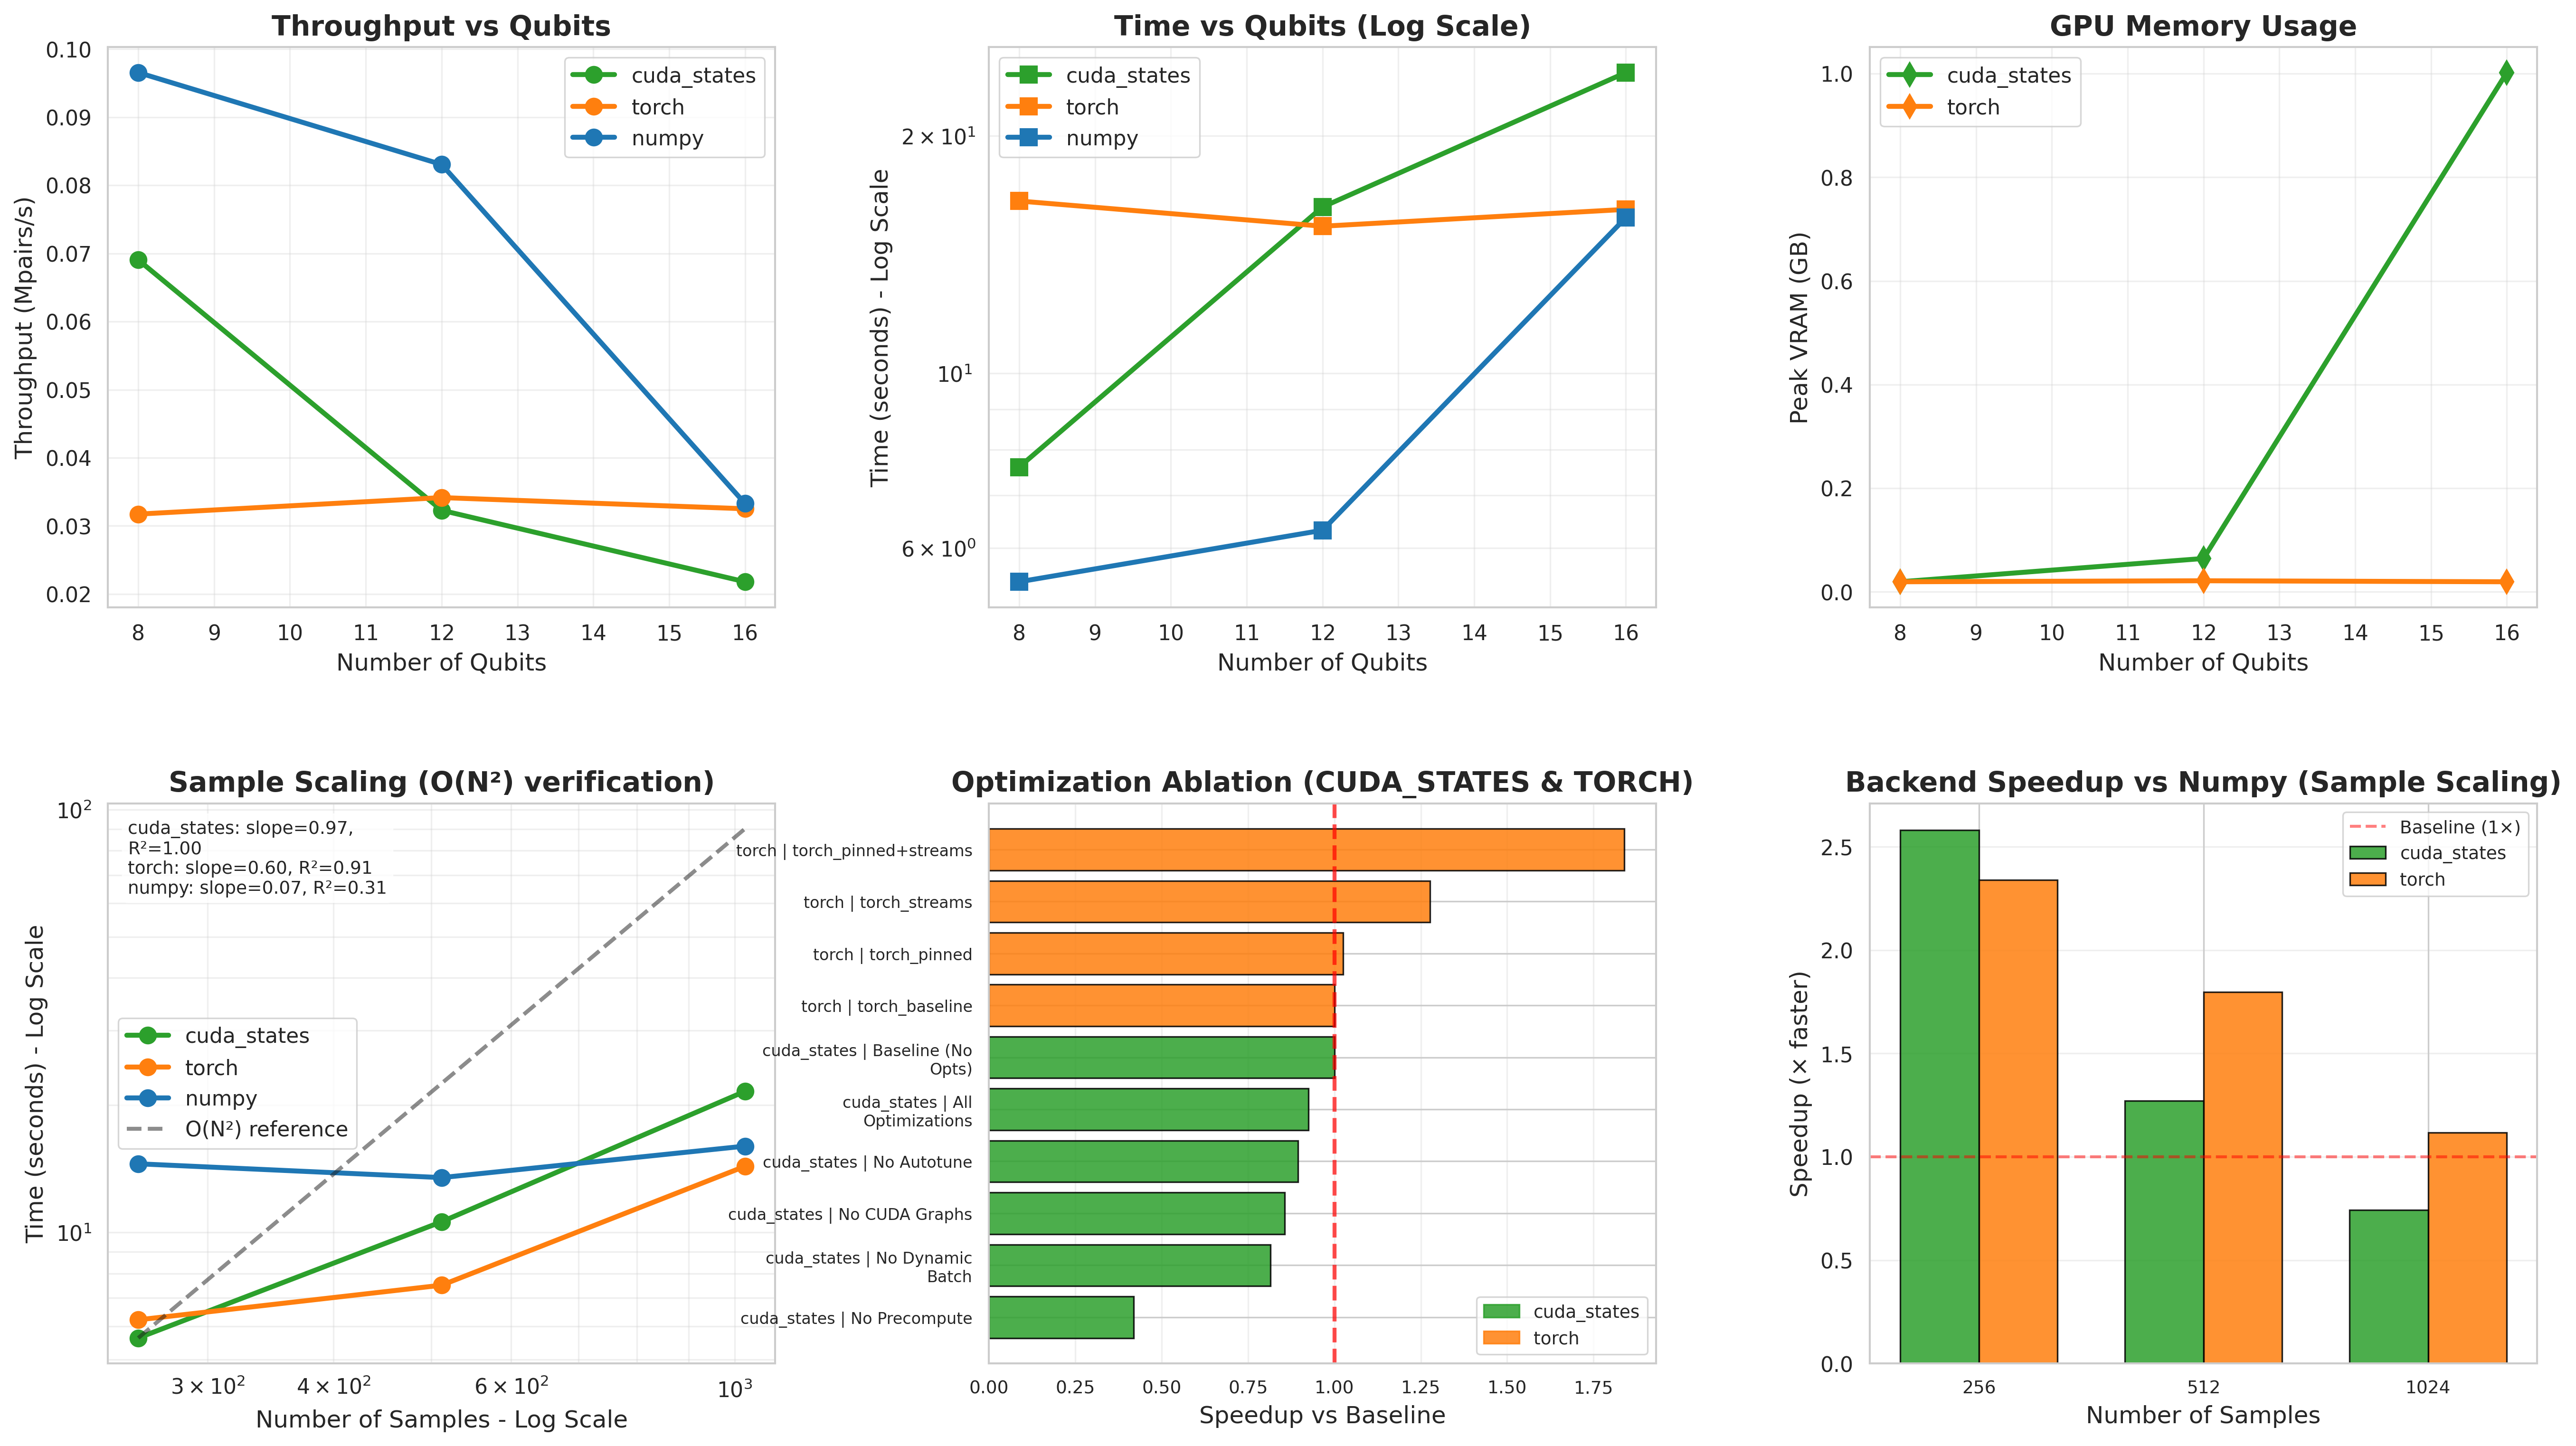
\includegraphics[width=\columnwidth]{benchmark_results/svhn/benchmark.png}
\caption{SVHN benchmark profile.}
\label{fig:bench-svhn}
\end{figure}

\FloatBarrier % Garde les figures dans cette section, mais autorise le texte suivant à monter sur la page !
% Le \clearpage a été supprimé d'ici pour éviter le saut de page forcé.


\section{Classification Results}
\begin{table}[t]
\centering
\caption{Quantum backend performance by dataset and sample size (mean over difficulty levels in the latest run-scoped extraction).}
\label{tab:classification-summary}
\scriptsize
\setlength{\tabcolsep}{3pt}
\resizebox{\columnwidth}{!}{%
\begin{tabular}{llcccc}
\toprule
\textbf{Dataset} & \textbf{Size} & \textbf{Backend} & \textbf{Mean F1} & \textbf{Mean AUC} & \textbf{Mean time (s)} \\
\midrule
cifar10 & 500  & \textbf{GPU custom} & 0.3500 & 0.4480 & 336.13 \\
cifar10 & 500  & \textbf{GPU base}   & 0.4270 & 0.4812 & 190.61 \\
cifar10 & 1000 & \textbf{GPU custom} & 0.4305 & 0.4365 & 496.73 \\
cifar10 & 1000 & \textbf{GPU base}   & 0.5729 & 0.5532 & 302.19 \\
fashion & 500  & \textbf{GPU custom} & 0.8905 & 0.9569 & 237.05 \\
fashion & 500  & \textbf{GPU base}   & 0.8889 & 0.9574 & 110.78 \\
fashion & 1000 & \textbf{GPU custom} & 0.8958 & 0.9553 & 339.29 \\
fashion & 1000 & \textbf{GPU base}   & 0.8998 & 0.9557 & 187.13 \\
svhn    & 500  & \textbf{GPU custom} & 0.1789 & 0.4719 & 545.39 \\
svhn    & 500  & \textbf{GPU base}   & 0.1547 & 0.4719 & 302.73 \\
svhn    & 1000 & \textbf{GPU custom} & 0.1596 & 0.4846 & 637.30 \\
svhn    & 1000 & \textbf{GPU base}   & 0.2998 & 0.4846 & 380.61 \\
\bottomrule
\end{tabular}
}
\end{table}

Table~\ref{tab:classification-summary} shows that, within quantum backends, \textbf{GPU base} is generally faster 
and often more accurate than \textbf{GPU custom}, while both remain strong on Fashion and weak on SVHN. Note that 
the reported \textbf{Mean time} measures the full pipeline execution, including state simulation, Gram matrix building, 
and the complete Optuna cross-validation loop.

\subsection{Quantum Comparison Against the Classical Baseline}

The comparison is performed on the shared setup (same dataset, same difficulty, and same sample sizes 500/1000).

The paired analysis is now stratified by sample size. 
Table~\ref{tab:latest-run-comparison} reports size-aware deltas.

\begin{table}[t]
\centering
\caption{Run-scoped paired comparison by sample size. Positive deltas indicate better classical quality; negative time deltas indicate 
faster classical execution.}
\label{tab:latest-run-comparison}
\scriptsize
\setlength{\tabcolsep}{4pt}
\resizebox{\columnwidth}{!}{%
\begin{tabular}{lccccc}
\toprule
\textbf{Comparison} & \textbf{Size} & $\Delta$\textbf{F1} & $\Delta$\textbf{AUC} & $\Delta$\textbf{Time (s)} & \textbf{Wins C/B/T} \\
\midrule
Classical $-$ GPU base & 500  & +0.1708 & +0.1488 & -188.28 & 8/0/1 \\
Classical $-$ GPU base & 1000 & +0.1721 & +0.1600 & -274.52 & 8/1/0 \\
Classical $-$ GPU custom & 500  & +0.1879 & +0.1600 & -359.76 & 8/0/1 \\
Classical $-$ GPU custom & 1000 & +0.2676 & +0.1990 & -475.66 & 8/1/0 \\
\bottomrule
\end{tabular}
}
\end{table}

Across both sizes, classical remains dominant in paired wins and runtime, while the size-wise split shows the gap is larger at 1000 samples than at 500.

\section{Failure Analysis: Kernel Collapse and Barren Plateau-Like Regimes}
Hard tasks exhibit the following quantitative pattern:
\begin{itemize}
    \item inter-class gap near zero after centering/normalization;
    \item test-kernel standard deviation on the order of $10^{-4}$ to $10^{-3}$;
    \item support-vector fraction near $1.0$;
    \item AUC close to 0.5 (random guessing) in the hardest cases.
\end{itemize}

The hard CIFAR-10 case with \textbf{6 layers} is particularly revealing. In this regime, one typically observes:
\begin{itemize}
    \item \textit{kernel std = 0.0005};
    \item \textit{SV frac = 1.0000};
    \item \textit{test F1 = 0.0000};
    \item \textit{test AUC = 0.4757}.
\end{itemize}

\begin{table}[t]
\centering
\caption{Difficulty-level summary across quantum backends (mean over datasets and sizes, latest run-scoped extraction).}
\label{tab:failure-difficulty}
\scriptsize
\setlength{\tabcolsep}{3pt}
\begin{tabular}{lccc}
\toprule
\textbf{Diff./Backend} & \textbf{F1} & \textbf{AUC} & \textbf{Time (s)} \\
\midrule
easy / GPU custom & 0.4907 & 0.6327 & 475.44 \\
easy / GPU base   & 0.6366 & 0.6499 & 258.76 \\
med / GPU custom  & 0.5263 & 0.6314 & 404.06 \\
med / GPU base    & 0.6560 & 0.6896 & 226.39 \\
hard / GPU custom & 0.4357 & 0.6125 & 416.44 \\
hard / GPU base   & 0.3289 & 0.6126 & 251.88 \\
\bottomrule
\end{tabular}
\end{table}

This behavior is consistent with a \textbf{kernel concentration}: states become almost indistinguishable in terms 
of overlap used by the SVM. It is reasonable to interpret this as a \emph{barren-plateau-like} or 
\emph{kernel collapse} regime~\cite{larocca2024review,thanasilp2022exponential}, 
although multiple factors likely combine:
\begin{itemize}
    \item loss of information due to conversion to grayscale and subsequent PCA;
    \item generic ansatz not informed by image geometry;
    \item increased depth favoring concentration of overlaps;
    \item intrinsic limitations of global fidelity kernels on complex visual data.
\end{itemize}

These observations indicate that acceleration alone does not remove the representational limits of the feature map.

\section{Data and Code Availability}
Project repository: \textbf{github.com/DylanUnifi}.

Datasets used in this study:
\begin{itemize}
    \item \textbf{Fashion-MNIST}~\cite{xiao2017fashion}.
    \item \textbf{CIFAR-10}~\cite{krizhevsky2009cifar}.
    \item \textbf{SVHN}~\cite{netzer2011svhn}.
\end{itemize}


\section{Conclusion}
The updated benchmark and classification tables show that backend ranking is not global: it depends on sample size, 
dataset profile, and backend implementation details.  In the benchmark campaign, GPU paths dominate low-size regimes, 
while some larger-size points still favor \textbf{CPU base} in specific profiles. On predictive quality, both quantum 
backends remain competitive on Fashion-MNIST but degrade on CIFAR-10 and especially SVHN, where collapse indicators 
and near-random AUC values appear repeatedly in hard settings. Overall, acceleration improves throughput but does not 
remove the representational bottleneck of the current feature map/ansatz pair on harder visual distributions.

\section{Perspectives}
Data-driven next steps are:
\begin{itemize}
    \item projected or local kernels to reduce global fidelity concentration effects;
    \item geometry-aware ansatz design tailored to image structure;
    \item stronger classical feature front-ends before PCA and quantum embedding;
    \item broader benchmark grids at fixed qubit counts per dataset;
    \item multi-GPU or MPI strategies to distribute one large Gram matrix build;
    \item native GPU-side SVM solvers to remove the final CPU training bottleneck;
    \item richer diagnostics (gap trajectories, spectra, support-vector dynamics) for earlier collapse detection.
\end{itemize}

{\small
\bibliographystyle{ieeetr}
\bibliography{parallel_qkernel_references}
}

\end{document}
